\section{Fallout3}

\begin{figure}[htbp]
\begin{center}
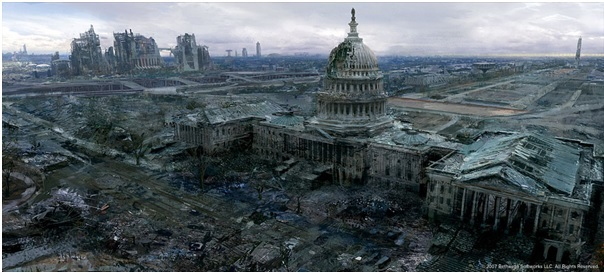
\includegraphics[width=.40\textwidth]{./imagenes/fallout3.jpg}
\caption{Fallout3}
\label{Fallout3}
\end{center}
\end{figure}
Fallout 3 tiene lugar en el año 2278, 200 años después de que una guerra mundial culminara en un holocausto nuclear. La ambientación consiste en una región post-apocalíptica y retrofuturista que abarca gran parte de Washington D.C., e  incluye edificios de la vida real devastados por la guerra como la Casa Blanca y el Monumento a Jefferson. El juego comienza dentro del Refugio 101, donde sus habitantes creen haber nacido originalmente, antes de aventurarse a las afueras del refugio donde se enfrentarán a la peligrosa verdad, un mundo devastado por la guerra, poblado por criaturas mutantes debido a los altos niveles de radiación.  

\subsubsection{¿Por qué es uno de mis juegos favoritos?}
\begin{itemize}
\item[José Salas] En Fallout 3, encarnamos a un niño que vive con su padre y el resto de una comunidad en un bunker, el Refugio 101. Totalmente aislados de los acontecimientos que se suceden en el exterior, y bajo una suerte de civilización con sus propias normas y leyes; la mayoría de sus ciudadanos han crecido ajenos a que en el exterior la tierra ha sido devastada por una guerra nuclear. El principal atractivo de Fallout 3 es el hecho de descubrirlo por nosotros mismos. Eventualmente salimos del refugio y vamos descubriendo este amplio mundo con total libertad.

\end{itemize}